\subsection{The attack}
In this section will follow the order established in the previous section, and will show screenshots of the executions described above. The figure \ref{fig:poc-tree} shows the general structure of this project, with the different files needed (the dependencies generated after \textit{npm install} have been omitted).\\
\begin{figure}[h]
    \centering
    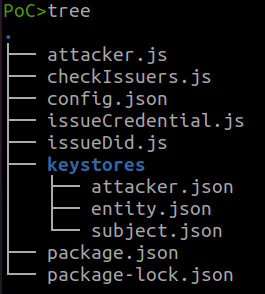
\includegraphics[width=0.4\textwidth]{images/PoC/tree.png}
    \caption{\acrshort{poc} tree}
    \label{fig:poc-tree}
\end{figure}

As already mentioned, we first visualize the roles of the entity and the attacker (1). The figure \ref{fig:poc-1} shows the output of the \textit{checkIssuers.js} script (listing \ref{lst:checkIssuers.js}). We can easily verify that the entity is an Issuer, but the attacker is not.\\
\begin{figure}[h]
    \centering
    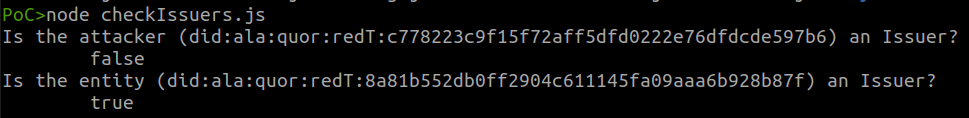
\includegraphics[width=1.0\textwidth]{images/PoC/1.png}
    \caption{checkIssuers.js output before the attack}
    \label{fig:poc-1}
\end{figure}

Then, from the entity we created a new identity (2) with the help of \textit{issueDid.js} (listing \ref{lst:issueDid.js}). We check that there is no problem when performing the service (figure \ref{fig:poc-2}).\\
\begin{figure}[h]
    \centering
    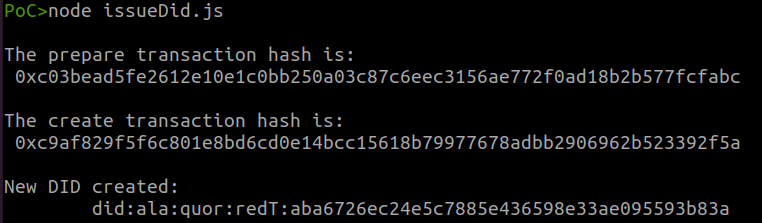
\includegraphics[width=1.0\textwidth]{images/PoC/2.png}
    \caption{issueDid.js output before the attack}
    \label{fig:poc-2}
\end{figure}

The third step is the attacker's turn (3), where using the \textit{attacker.js} script (listing \ref{lst:attacker.js}). This output (figure \ref{fig:poc-3}) does not provide anything interesting, except the hash of the transaction made.\\
\begin{figure}[h]
    \centering
    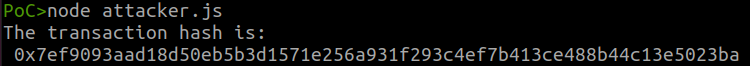
\includegraphics[width=1.0\textwidth]{images/PoC/3.png}
    \caption{attacker.js output}
    \label{fig:poc-3}
\end{figure}

To verify that the attack has been successful (4), we run the Issuer status check on the entity and the attacker again (figure \ref{fig:poc-4}). This time we see that the entity (\acrshort{did} "did:ala:quor:redT:8a81b552db0ff2904c611145fa09aaa6b928b87f") is not an Issuer.\\
% TODO muy pequeña, recortar y agrandar
\begin{figure}[h]
    \centering
    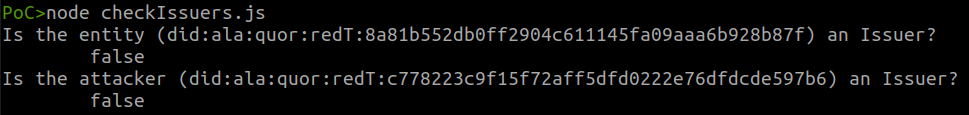
\includegraphics[width=1.0\textwidth]{images/PoC/4.png}
    \caption{checkIssuers.js output after the attack}
    \label{fig:poc-4}
\end{figure}

The last check that is made, is to try again to create an identity again (5). For this, we run again \textit{issueDid.js} (listing \ref{lst:issueDid.js}), but now in the output (figure \ref{fig:poc-5}) we see an error \textit{"ERROR prepare: Error: Transaction has been reverted by the EVM"}. This error indicates that the \textit{"prepare"} transaction, that is the first one of two that is made for the identity creation, has failed. This is because now the entity does not satisfy the modifier of the function \textit{prepareAlastriaID} of the Smart Contract \textit{AlastriaIdentityManager.sol}\footnote{\url{https://github.com/alastria/alastria-identity/blob/master/contracts/identityManager/AlastriaIdentityManager.sol\#L52}}. The modifier requires that the function caller has the Issuer role.
\begin{figure}[h]
    \centering
    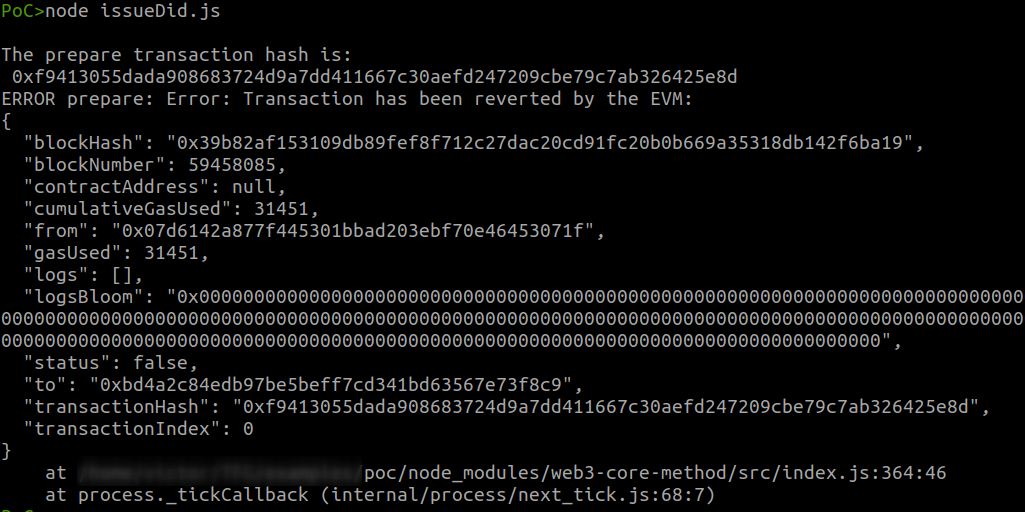
\includegraphics[width=1.0\textwidth]{images/PoC/5.png}
    \caption{issueDid.js output after the attack}
    \label{fig:poc-5}
\end{figure}
